\section{Live User Collaboration}
\label{prototype:LiveUserCollaboration}
Collaboration is one of the core pillars therefore for this first software test I decided to experiment with real time collaboration using the socket IO technology I previously researched. At this point I haven't completed my research on web hosting platforms / technologies so I utilised this code I had put together following a mix of tutorial and trial by error.

\begin{figure}[H]
    \centering
    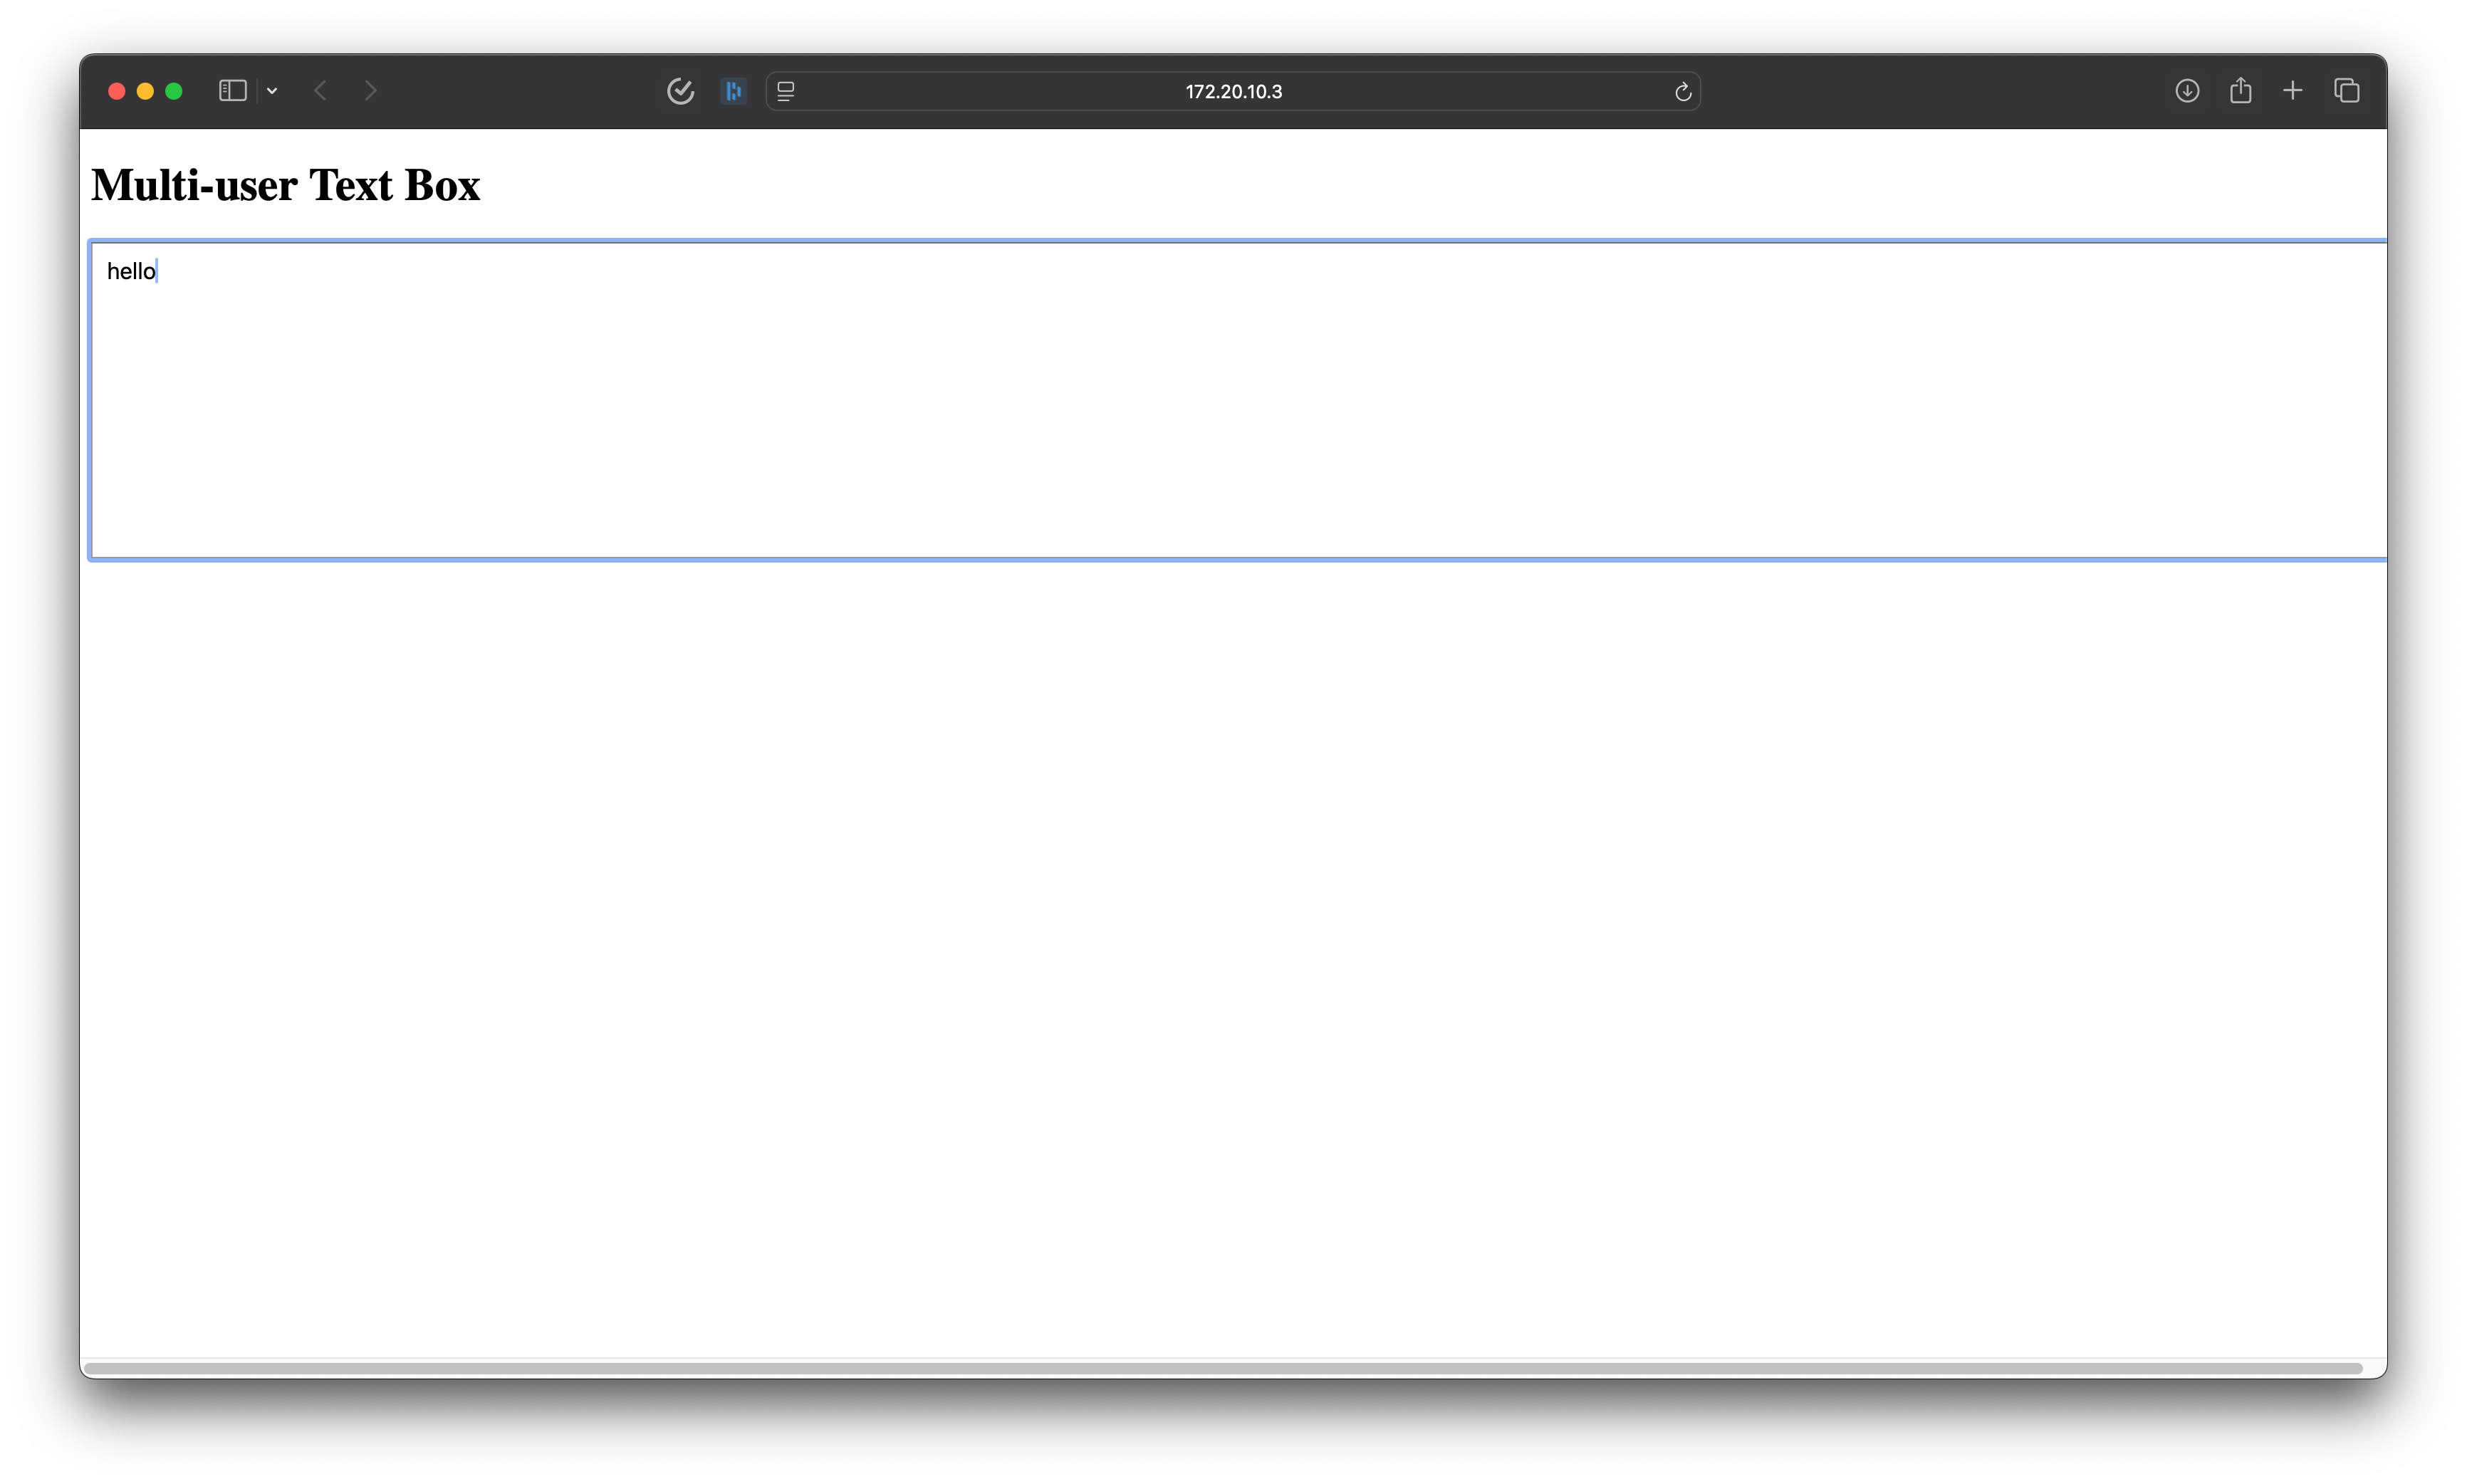
\includegraphics[width=0.8\textwidth]{Prototype/7_TextCollaboration/media/prototype.png}
    \caption{Live User Collaboration Prototype}
    \label{fig:LiveUserCollaborationPrototype}
\end{figure}
\subsection*{Python Code}
This code is a simple web server that allows multiple users to connect and send messages in real-time.
\inputminted[linenos, tabsize=1, breaklines]{python}{Prototype/7_TextCollaboration/media/PythonCode.py}

\subsection*{HTML Code}
This code runs on the clients device in the browser and connects to the Python server, allowing users to send and receive messages
\inputminted[linenos, tabsize=1, breaklines]{html}{Prototype/7_TextCollaboration/media/HtmlCode.html}
